\chapter{Conception et réalisation matérielle}

\tikzset{
  annot/.style={draw=orangefst,very thick,{Circle[length=4.5pt,fill=orangefst]}-},
  lab/.style={font=\scriptsize,fill=white,draw=orangefst!60,rounded corners=2pt,inner sep=2.5pt,align=left},
}

\section{Introduction}
Ce chapitre décrit la partie matérielle du projet : la voiture miniature qui constitue l'environnement
\emph{prototype}. Nous présentons d'abord l'architecture matérielle d'ensemble, puis chacun des composants
(rôle, caractéristiques et broches utilisées), le système d'alimentation, le schéma de câblage et enfin la
réalisation physique du prototype et de sa piste.

% ------------------------------------------------------------------------------------------------
\section{Architecture matérielle du système}

Le prototype est organisé autour de deux sous-systèmes indépendants (figure~\ref{fig:archi-materielle}) :
\begin{itemize}
  \item \textbf{le sous-système de commande}, construit autour de l'Arduino UNO, qui lit les capteurs infrarouges
        et ultrasonique et commande les deux moteurs à travers le pont en H L298N. Il assure de manière autonome
        le suivi de la piste et l'arrêt devant un obstacle ;
  \item \textbf{le sous-système de vision}, formé de l'ESP32-CAM montée sur sa carte ESP32-CAM-MB et alimentée par
        une batterie externe. Il filme la route et diffuse les images en Wi-Fi vers le serveur \app.
\end{itemize}
Les deux sous-systèmes ne sont pas reliés entre eux : il n'existe pas de liaison série entre l'Arduino et
l'ESP32-CAM. Toutes les informations du prototype affichées par l'application proviennent donc de l'image.

\begin{figure}[H]
\centering
\resizebox{\linewidth}{!}{%
\begin{tikzpicture}[node distance=0.5cm and 0.9cm,
  pw/.style={-{Stealth[length=2.4mm]},very thick,draw=critique!85},
  sg/.style={-{Stealth[length=2.4mm]},thick,draw=bleufst},
  lb/.style={font=\scriptsize,fill=white,inner sep=1pt}]
  \node[bloco,minimum width=2.6cm] (bat) {4 piles AA\\($\approx$ 6 V)};
  \node[bloco,minimum width=2.6cm,below=0.9cm of bat] (sw) {Interrupteur};
  \node[blocg,minimum width=3cm,minimum height=2.2cm,right=1.6cm of sw] (l298) {Pont en H\\L298N};
  \node[bloc,minimum width=2.6cm,above right=0.2cm and 1.2cm of l298] (mg) {Moteur gauche};
  \node[bloc,minimum width=2.6cm,below right=0.2cm and 1.2cm of l298] (md) {Moteur droit};
  \node[blocg,minimum width=3.4cm,minimum height=2.4cm,below=2.2cm of l298] (uno) {Arduino UNO\\ATmega328P};
  \node[bloc,minimum width=2.6cm,left=2.2cm of uno.north west,anchor=north east] (irg) {Capteur IR gauche};
  \node[bloc,minimum width=2.6cm,below=0.35cm of irg] (ird) {Capteur IR droit};
  \node[bloc,minimum width=2.6cm,below=0.35cm of ird] (us) {HC-SR04};
  \node[bloco,minimum width=3cm,right=1.7cm of mg] (pb) {Batterie externe\\5 V (USB)};
  \node[bloc,minimum width=3cm,below=0.9cm of pb] (mb) {ESP32-CAM-MB\\(USB / programmation)};
  \node[blocg,minimum width=3cm,below=0.5cm of mb] (cam) {ESP32-CAM\\caméra OV3660};
  \node[bloc,draw=gris,minimum width=3cm,below=1.3cm of cam] (srv) {Serveur \app\\(ordinateur portable)};
  % alimentation
  \draw[pw] (bat) -- node[lb,right] {+} (sw);
  \draw[pw] (sw) -- node[lb,above] {VS} (l298);
  \draw[pw] (pb) -- node[lb,right] {5 V} (mb);
  \draw[pw,dashed] (pb.south west) to[out=-120,in=0] node[lb,pos=0.7,below] {5 V (USB)} (uno.east);
  \draw[pw] (mb) -- (cam);
  \draw[pw,{Stealth[length=2.4mm]}-{Stealth[length=2.4mm]}] (l298.south) -- node[lb,right] {5 V / GND communs} (uno.north);
  % moteurs
  \draw[sg,draw=encre] (l298.east) ++(0,0.4) -- node[lb,above,sloped] {OUT1--OUT2} (mg.west);
  \draw[sg,draw=encre] (l298.east) ++(0,-0.4) -- node[lb,below,sloped] {OUT3--OUT4} (md.west);
  % signaux
  \draw[sg] (irg.east) -- node[lb,above] {D2} (irg.east -| uno.west);
  \draw[sg] (ird.east) -- node[lb,above] {D3} (ird.east -| uno.west);
  \draw[sg,{Stealth[length=2.4mm]}-{Stealth[length=2.4mm]}] (us.east) -- node[lb,above] {D12 Trig / D13 Echo} (us.east -| uno.west);
  \draw[sg] ([xshift=0.8cm]uno.north) -- node[lb,right] {D8--D11 $\rightarrow$ IN1--IN4} ([xshift=0.8cm]l298.south);
  % wifi
  \draw[sg,dashed,draw=vertfst!70!black] (cam) -- node[lb,right] {Wi-Fi : flux MJPEG} (srv);
  \begin{scope}[on background layer]
    \node[zone,fill=bleufst!4,fit=(bat)(l298)(mg)(md)(uno)(irg)(us),label={[font=\bfseries\small]above:Sous-système de commande}] {};
    \node[zone,fill=vertfst!5,fit=(pb)(mb)(cam),label={[font=\bfseries\small]above:Sous-système de vision}] {};
  \end{scope}
  \node[font=\scriptsize,align=left,anchor=north west] at ($(us.south west)+(0,-0.5)$)
    {\textcolor{critique}{\rule[2pt]{0.6cm}{1.4pt}} alimentation \quad \textcolor{bleufst}{\rule[2pt]{0.6cm}{1.2pt}} signaux
     \quad \textcolor{vertfst!70!black}{- - -} liaison sans fil};
\end{tikzpicture}}
\caption{Architecture matérielle du prototype}
\label{fig:archi-materielle}
\end{figure}

Le tableau~\ref{tab:composants} récapitule les composants utilisés.

\begin{table}[H]
\centering\small
\caption{Composants du prototype}
\label{tab:composants}
\begin{tabularx}{\linewidth}{l c X}
\toprule
\textbf{Composant} & \textbf{Qté} & \textbf{Rôle} \\
\midrule
Arduino UNO (ATmega328P)          & 1 & Unité de commande : lecture des capteurs, commande des moteurs \\
Module L298N (double pont en H)   & 1 & Interface de puissance entre l'Arduino et les moteurs \\
Moteur à courant continu avec réducteur (« TT ») & 2 & Propulsion et direction différentielle \\
Capteur infrarouge à réflexion    & 2 & Détection du ruban noir de la piste (gauche / droite) \\
Capteur ultrasonique HC-SR04      & 1 & Mesure de la distance à l'obstacle frontal \\
ESP32-CAM + carte ESP32-CAM-MB    & 1 & Acquisition et diffusion Wi-Fi des images \\
4 piles alcalines AA 1,5 V + interrupteur & 1 & Alimentation des moteurs \\
Batterie externe USB 5 V          & 1 & Alimentation de la caméra et de l'électronique de commande \\
Châssis, roues, roue folle, fils Dupont & — & Structure mécanique et liaisons \\
\bottomrule
\end{tabularx}
\end{table}

% ------------------------------------------------------------------------------------------------
\section{Arduino UNO}

L'Arduino UNO est une carte de développement construite autour du microcontrôleur 8 bits ATmega328P de
Microchip~\cite{arduinouno}. Elle est simple à programmer (langage Arduino, dérivé du C++), robuste et bien
documentée, ce qui en fait un choix naturel pour la boucle de commande du prototype. Ses principales
caractéristiques sont données dans le tableau~\ref{tab:uno}, et la figure~\ref{fig:uno} identifie ses broches
principales.

\begin{table}[H]
\centering\small
\caption{Caractéristiques principales de l'Arduino UNO}
\label{tab:uno}
\begin{tabular}{ll}
\toprule
Microcontrôleur & ATmega328P, 8 bits, 16 MHz \\
Mémoires & 32 Ko de Flash, 2 Ko de SRAM, 1 Ko d'EEPROM \\
Entrées / sorties numériques & 14 (dont 6 compatibles MLI/PWM) \\
Entrées analogiques & 6 (A0 à A5), convertisseur 10 bits \\
Tension de fonctionnement & 5 V (alimentation par USB ou prise jack 7--12 V) \\
Courant maximal par broche & 20 mA recommandés (40 mA absolus) \\
\bottomrule
\end{tabular}
\end{table}

\begin{figure}[H]
\centering
\begin{tikzpicture}
  \node[anchor=south west,inner sep=0] (img) at (0,0) {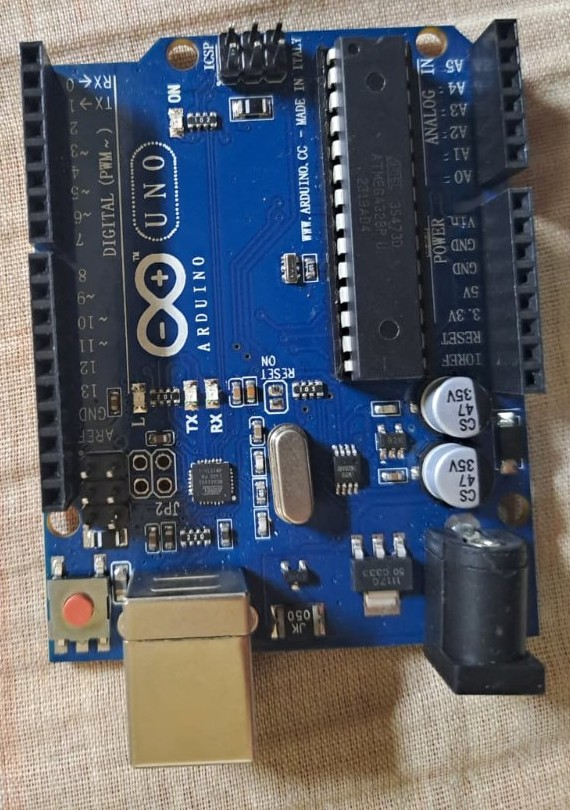
\includegraphics[width=5.4cm]{photos/arduino_uno_crop.jpg}};
  \begin{scope}[x={(img.south east)},y={(img.north west)}]
    \draw[annot] (0.06,0.83) -- (-0.12,0.83) node[lab,left] {Broches numériques D0--D7\\(D2, D3 : capteurs IR)};
    \draw[annot] (0.06,0.57) -- (-0.12,0.57) node[lab,left] {Broches D8--D13\\(D8--D11 : L298N ; D12, D13 : HC-SR04)};
    \draw[annot] (0.135,0.247) -- (-0.12,0.30) node[lab,left] {Bouton de réinitialisation};
    \draw[annot] (0.325,0.13) -- (-0.12,0.08) node[lab,left] {Port USB-B\\(programmation, alimentation)};
    \draw[annot] (0.447,0.93) -- (1.12,0.97) node[lab,right] {Connecteur ICSP};
    \draw[annot] (0.66,0.74) -- (1.12,0.78) node[lab,right] {Microcontrôleur\\ATmega328P};
    \draw[annot] (0.895,0.877) -- (1.12,0.88) node[lab,right] {Entrées analogiques A0--A5};
    \draw[annot] (0.91,0.654) -- (1.12,0.60) node[lab,right] {Alimentation :\\5 V, 3,3 V, GND, Vin};
    \draw[annot] (0.51,0.42) -- (1.12,0.42) node[lab,right] {Quartz 16 MHz};
    \draw[annot] (0.85,0.235) -- (1.12,0.22) node[lab,right] {Prise jack (7--12 V)};
  \end{scope}
\end{tikzpicture}
\caption{Carte Arduino UNO du prototype et ses broches principales}
\label{fig:uno}
\end{figure}

Dans notre montage, l'Arduino utilise huit broches numériques (tableau~\ref{tab:broches}). Les broches D2 et D3
reçoivent les sorties tout-ou-rien des capteurs infrarouges ; D8 à D11 imposent le sens de rotation des moteurs
au L298N ; D12 déclenche la mesure du HC-SR04 et D13 en reçoit l'écho.

\begin{table}[H]
\centering\small
\caption{Affectation des broches de l'Arduino UNO}
\label{tab:broches}
\begin{tabular}{lll}
\toprule
\textbf{Broche} & \textbf{Connectée à} & \textbf{Rôle} \\
\midrule
D2  & Capteur IR gauche (OUT) & Entrée : ruban détecté à gauche \\
D3  & Capteur IR droit (OUT)  & Entrée : ruban détecté à droite \\
D8, D9 & L298N IN1, IN2 & Sorties : sens du moteur gauche \\
D10, D11 & L298N IN3, IN4 & Sorties : sens du moteur droit \\
D12 & HC-SR04 Trig & Sortie : impulsion de déclenchement (10 µs) \\
D13 & HC-SR04 Echo & Entrée : durée de l'écho \\
5 V, GND & L298N, HC-SR04, capteurs IR & Alimentation logique et masse commune \\
\bottomrule
\end{tabular}
\end{table}

% ------------------------------------------------------------------------------------------------
\section{Module L298N}

Un microcontrôleur ne peut fournir que quelques dizaines de milliampères par broche, alors qu'un moteur en
consomme plusieurs centaines. Le module L298N sert d'interface de puissance : il contient deux ponts en H qui
permettent de commander indépendamment le sens (et, par les entrées ENA/ENB, la vitesse) de deux moteurs à courant
continu~\cite{l298}. Il accepte une tension moteur de 5 à 35 V, un courant de 2 A par voie, et intègre un
régulateur 5 V (78M05). Les bornes et entrées du module sont identifiées sur la figure~\ref{fig:l298n}.

\begin{figure}[H]
\centering
\begin{tikzpicture}
  \node[anchor=south west,inner sep=0] (img) at (0,0) {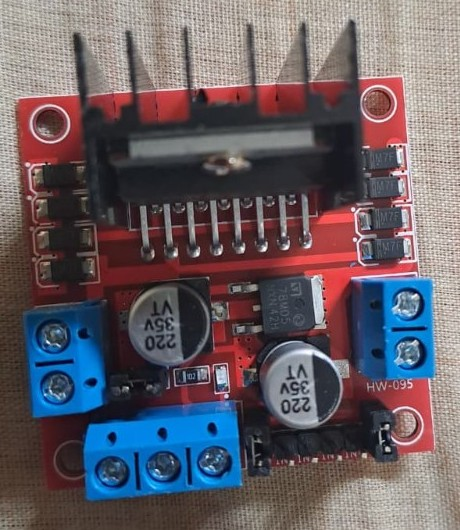
\includegraphics[width=6cm]{photos/l298n_crop.jpg}};
  \begin{scope}[x={(img.south east)},y={(img.north west)}]
    \draw[annot] (0.478,0.736) -- (1.1,0.86) node[lab,right] {Circuit L298N\\et son radiateur};
    \draw[annot] (0.63,0.415) -- (1.1,0.66) node[lab,right] {Régulateur 5 V (78M05)};
    \draw[annot] (0.859,0.377) -- (1.1,0.45) node[lab,right] {Sortie moteur B\\(OUT3, OUT4) $\rightarrow$ moteur droit};
    \draw[annot] (0.696,0.155) -- (1.1,0.16) node[lab,right] {Entrées IN1--IN4\\et cavaliers ENA / ENB};
    \draw[annot] (0.141,0.32) -- (-0.1,0.48) node[lab,left] {Sortie moteur A\\(OUT1, OUT2) $\rightarrow$ moteur gauche};
    \draw[annot] (0.289,0.274) -- (-0.1,0.28) node[lab,left] {Cavalier d'activation\\du régulateur 5 V};
    \draw[annot] (0.352,0.132) -- (-0.1,0.08) node[lab,left] {Bornier d'alimentation :\\VS (+6 V), GND, +5 V};
  \end{scope}
\end{tikzpicture}
\caption{Module L298N : bornes d'alimentation, entrées de commande et sorties moteurs}
\label{fig:l298n}
\end{figure}

Les cavaliers ENA et ENB étant en place, les deux moteurs tournent à pleine tension et leur sens est fixé par les
entrées IN (tableau~\ref{tab:l298}). La direction de la voiture est obtenue par \emph{commande différentielle} :
pour tourner à gauche, on ralentit ou on arrête le moteur gauche pendant que le moteur droit continue d'avancer.

\begin{table}[H]
\centering\small
\caption{Commande d'un moteur par le L298N (moteur gauche : IN1/IN2 ; moteur droit : IN3/IN4)}
\label{tab:l298}
\begin{tabular}{ccl}
\toprule
\textbf{IN1 (IN3)} & \textbf{IN2 (IN4)} & \textbf{Effet sur le moteur} \\
\midrule
1 & 0 & Rotation en marche avant \\
0 & 1 & Rotation en marche arrière \\
0 & 0 & Roue libre (arrêt) \\
1 & 1 & Freinage \\
\bottomrule
\end{tabular}
\end{table}

Il faut noter que le L298N, à transistors bipolaires, provoque une chute de tension de l'ordre de 2 V : avec une
alimentation de 6 V, les moteurs reçoivent environ 4 V, ce qui limite la vitesse de la voiture.

% ------------------------------------------------------------------------------------------------
\section{Moteurs à courant continu}

La propulsion est assurée par deux moteurs à courant continu munis d'un réducteur en plastique (moteurs dits
« TT », figure~\ref{fig:moteurs}). Prévus pour 3 à 6 V, ils offrent, grâce au réducteur (rapport typique 1:48), un
couple suffisant pour entraîner directement les roues de 65 mm. Chaque moteur est fixé sur le châssis par un
support et entraîne une roue arrière ; une roue folle à l'avant assure l'équilibre. Les deux moteurs étant
commandés séparément, la voiture tourne en faisant varier la vitesse relative des deux roues.

\begin{figure}[H]
\centering
\begin{subfigure}[b]{0.3\linewidth}\centering
  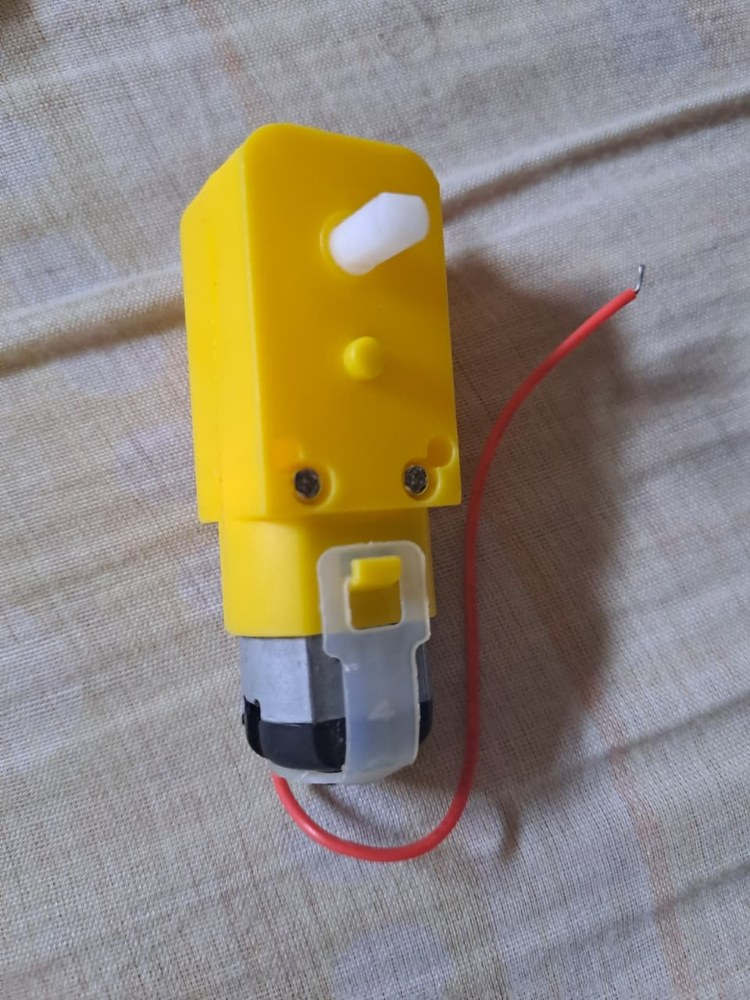
\includegraphics[height=5.2cm]{photos/moteur_tt.jpg}
  \caption{Moteur à réducteur (identique pour les deux côtés)}
\end{subfigure}\hspace{1cm}
\begin{subfigure}[b]{0.3\linewidth}\centering
  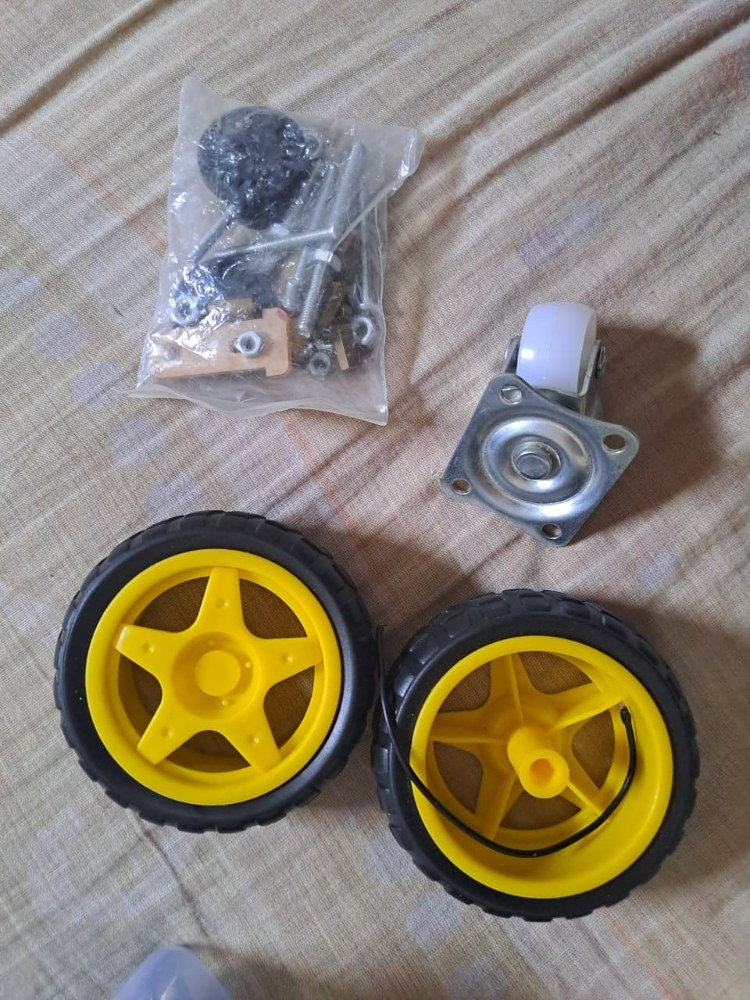
\includegraphics[height=5.2cm]{photos/roues.jpg}
  \caption{Roues, roue folle et visserie}
\end{subfigure}
\caption{Les deux moteurs à courant continu et les éléments de roulement}
\label{fig:moteurs}
\end{figure}

% ------------------------------------------------------------------------------------------------
\section{Capteurs infrarouges}

Deux capteurs infrarouges à réflexion, orientés vers le sol, permettent de suivre la piste (figure~\ref{fig:ir}).
Chaque module comporte une LED émettrice infrarouge, une photodiode réceptrice, un comparateur LM393 et un
potentiomètre de réglage du seuil. Le sol clair réfléchit le rayonnement infrarouge, alors que le ruban noir
l'absorbe : la sortie numérique OUT change donc d'état lorsque le capteur passe au-dessus du ruban. Le
potentiomètre permet d'ajuster le seuil à la hauteur du capteur et à l'éclairage.

\begin{figure}[H]
\centering
\begin{subfigure}[b]{0.3\linewidth}\centering
  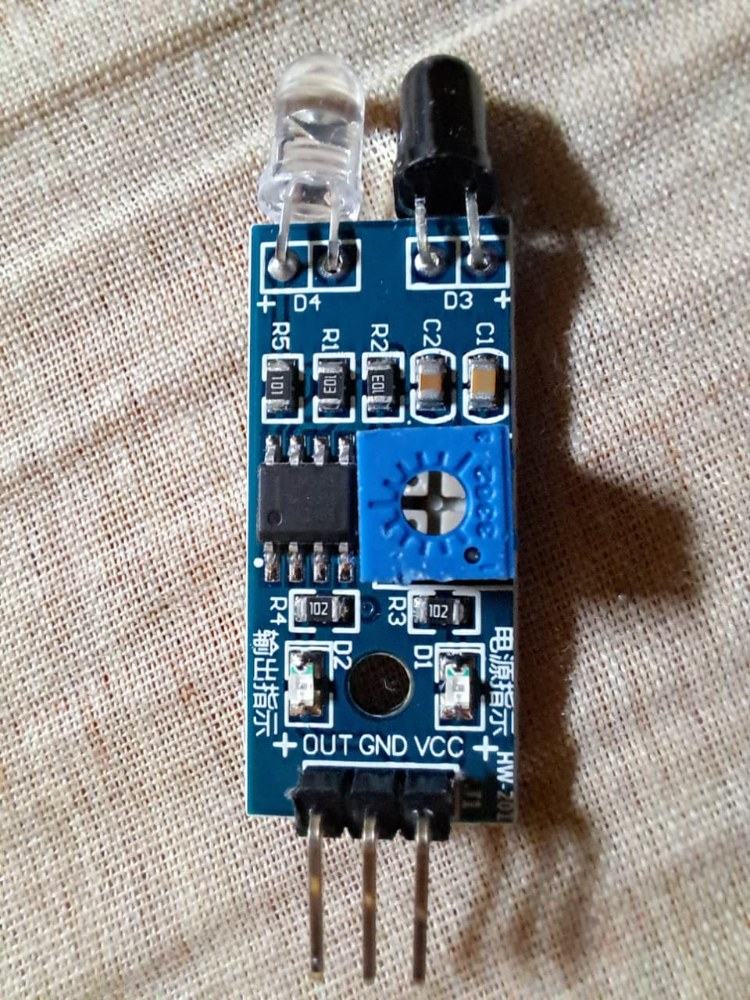
\includegraphics[height=5.6cm]{photos/ir_face.jpg}
  \caption{Face avant : LED IR, photodiode, potentiomètre, broches OUT / GND / VCC}
\end{subfigure}\hspace{1cm}
\begin{subfigure}[b]{0.3\linewidth}\centering
  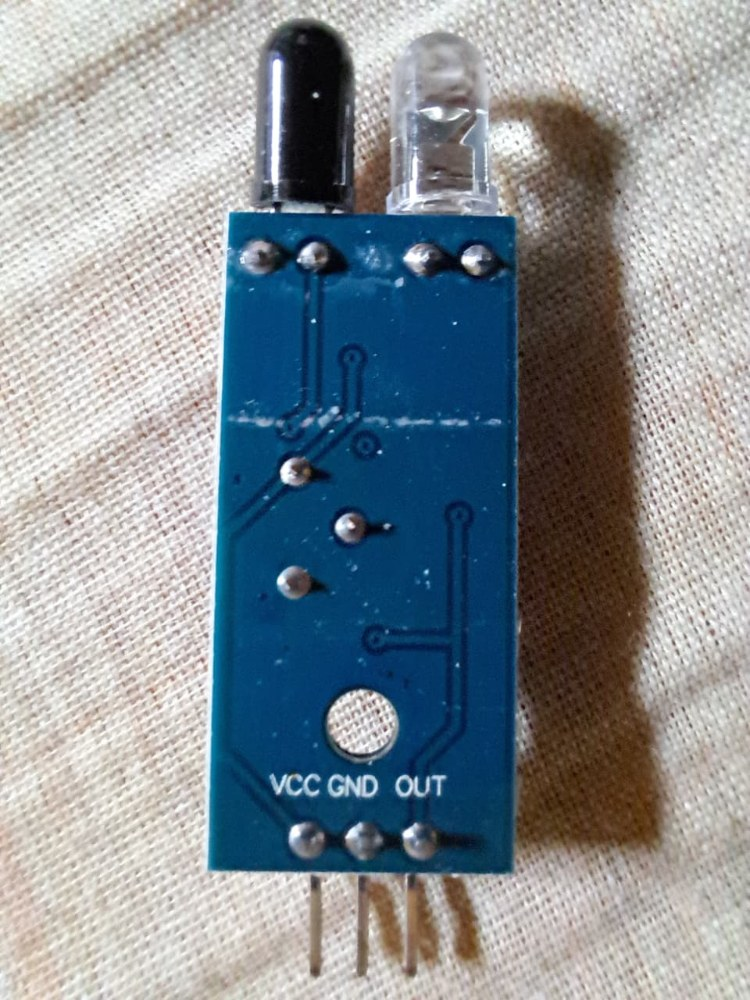
\includegraphics[height=5.6cm]{photos/ir_dos.jpg}
  \caption{Face arrière}
\end{subfigure}
\caption{Capteurs infrarouges gauche et droit (deux modules identiques)}
\label{fig:ir}
\end{figure}

Les deux capteurs sont placés de part et d'autre du ruban. Tant que tous deux voient le sol clair, la voiture
avance tout droit ; lorsque l'un d'eux détecte le ruban, la ligne s'est décalée de ce côté et la voiture tourne
dans cette direction (tableau~\ref{tab:suivi}).

\begin{table}[H]
\centering\small
\caption{Logique de suivi de ligne à deux capteurs}
\label{tab:suivi}
\begin{tabular}{ccl}
\toprule
\textbf{IR gauche} & \textbf{IR droit} & \textbf{Action} \\
\midrule
sol clair & sol clair & Avancer tout droit \\
ruban noir & sol clair & Tourner à gauche \\
sol clair & ruban noir & Tourner à droite \\
ruban noir & ruban noir & S'arrêter (croisement ou fin de piste) \\
\bottomrule
\end{tabular}
\end{table}

% ------------------------------------------------------------------------------------------------
\section{Capteur ultrasonique HC-SR04}

Le HC-SR04 mesure la distance à l'obstacle situé devant la voiture par temps de vol d'une onde ultrasonore
(figure~\ref{fig:hcsr04})~\cite{hcsr04}. Une impulsion d'au moins 10 µs sur la broche \textbf{Trig} déclenche
l'émission d'une salve de huit impulsions à 40 kHz ; la broche \textbf{Echo} passe alors à l'état haut pendant
une durée $t$ égale au temps d'aller-retour de l'onde. La distance s'en déduit par :
\begin{equation}
  d = \frac{v_{son}\, t}{2} \approx \frac{343~\text{m/s} \times t}{2}
  \quad\Longleftrightarrow\quad d~[\text{cm}] \approx \frac{t~[\text{µs}]}{58}
\end{equation}
Le capteur mesure de 2 cm à 4 m environ, avec un cône de détection d'une quinzaine de degrés. Il est alimenté en
5 V et ses quatre broches sont : \textbf{VCC}, \textbf{Trig}, \textbf{Echo} et \textbf{GND}.

\begin{figure}[H]
\centering
\begin{tikzpicture}
  \node[anchor=south west,inner sep=0] (img) at (0,0) {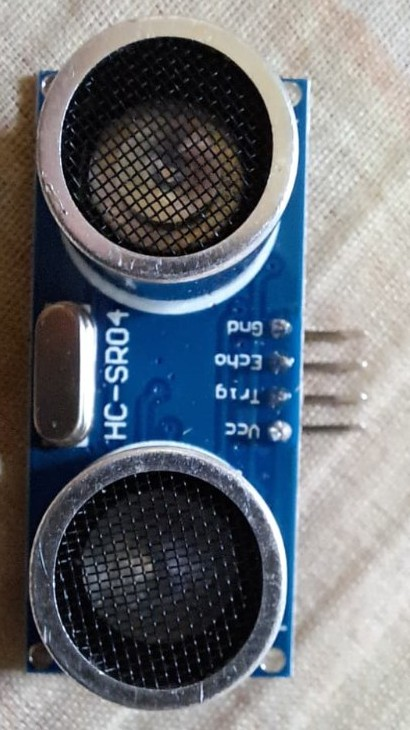
\includegraphics[width=3.9cm]{photos/hcsr04_crop.jpg}};
  \begin{scope}[x={(img.south east)},y={(img.north west)}]
    \draw[annot] (0.878,0.544) -- (1.25,0.70) node[lab,right] {\textbf{GND} — masse};
    \draw[annot] (0.878,0.501) -- (1.25,0.59) node[lab,right] {\textbf{Echo} $\rightarrow$ D13 (durée de l'écho)};
    \draw[annot] (0.878,0.459) -- (1.25,0.48) node[lab,right] {\textbf{Trig} $\leftarrow$ D12 (impulsion de 10 µs)};
    \draw[annot] (0.878,0.416) -- (1.25,0.37) node[lab,right] {\textbf{VCC} — alimentation 5 V};
    \draw[annot] (0.40,0.80) -- (-0.15,0.80) node[lab,left] {Transducteur ultrasonore\\(40 kHz)};
    \draw[annot] (0.38,0.22) -- (-0.15,0.22) node[lab,left] {Transducteur ultrasonore\\(40 kHz)};
    \draw[annot] (0.16,0.49) -- (-0.15,0.51) node[lab,left] {Oscillateur à quartz};
  \end{scope}
\end{tikzpicture}
\caption{Capteur ultrasonique HC-SR04 et ses quatre broches}
\label{fig:hcsr04}
\end{figure}

% ------------------------------------------------------------------------------------------------
\section{ESP32-CAM}

L'ESP32-CAM (modèle AI-Thinker) est un module très compact qui associe un microcontrôleur ESP32 à double cœur
(240 MHz) doté du Wi-Fi et du Bluetooth, 4 Mo de mémoire PSRAM, un connecteur de caméra, un lecteur de carte
microSD et une LED de flash~\cite{esp32cam}. Le module de notre prototype porte un capteur OV3660 ; il ne
possède pas de port USB et se programme à travers sa carte support \textbf{ESP32-CAM-MB}, qui lui fournit une
interface USB-série (CH340), des boutons de démarrage et de réinitialisation, et l'alimentation 5 V
(figure~\ref{fig:esp32cam}).

\begin{figure}[H]
\centering
\begin{subfigure}[b]{0.31\linewidth}\centering
  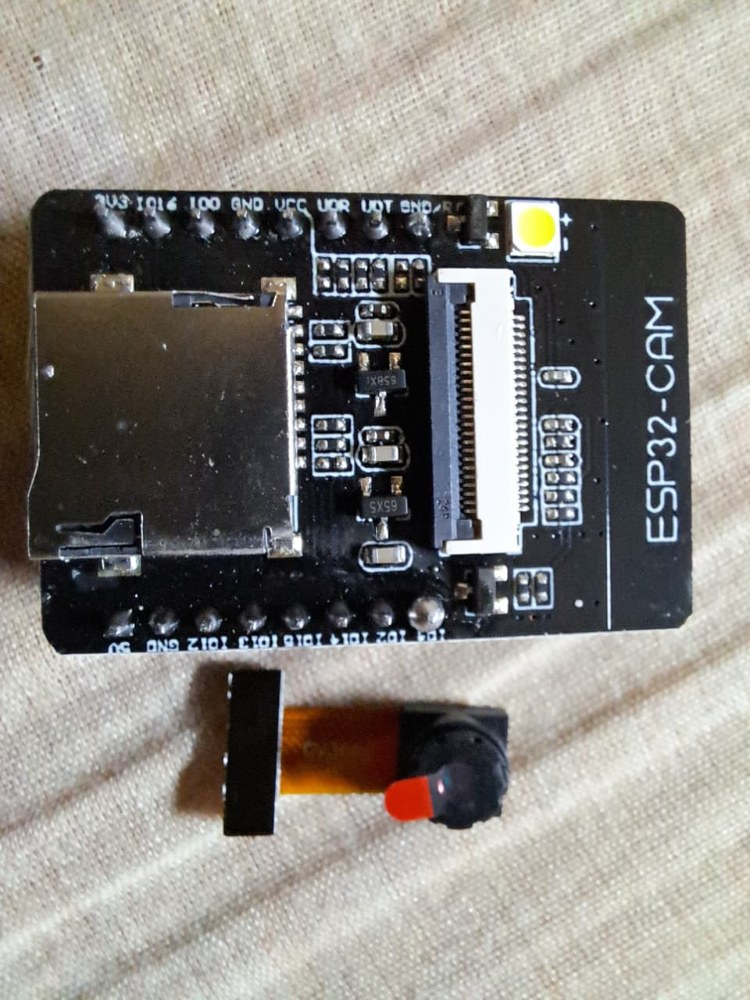
\includegraphics[height=5.4cm]{photos/esp32cam.jpg}
  \caption{Module ESP32-CAM et sa caméra}
\end{subfigure}\hfill
\begin{subfigure}[b]{0.31\linewidth}\centering
  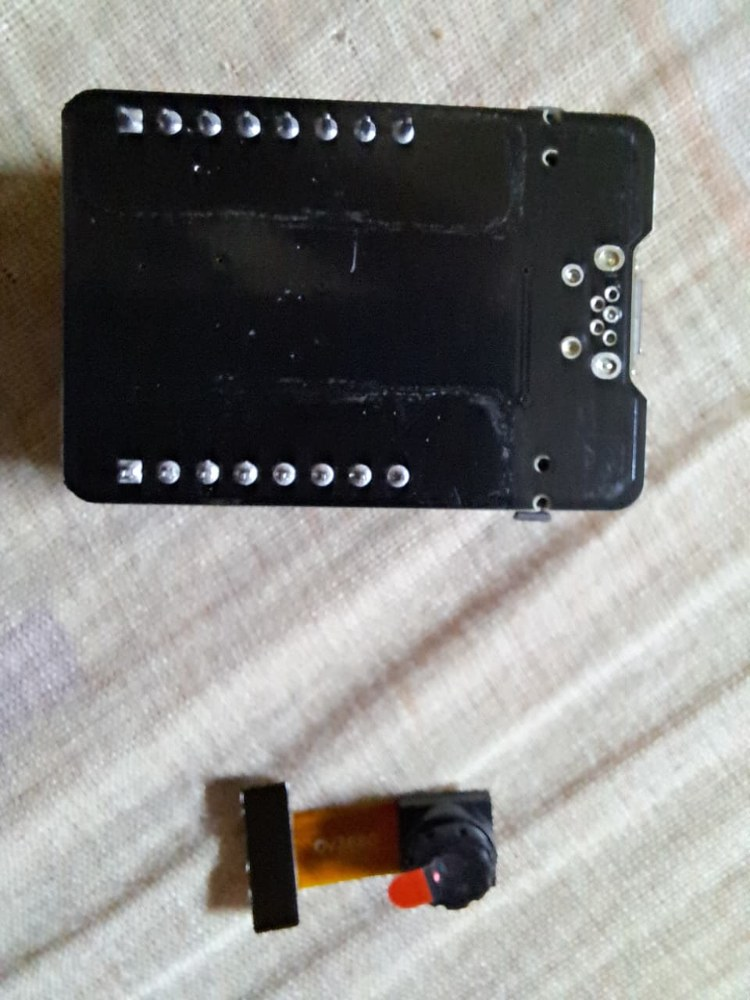
\includegraphics[height=5.4cm]{photos/esp32cam_mb.jpg}
  \caption{Carte support ESP32-CAM-MB}
\end{subfigure}\hfill
\begin{subfigure}[b]{0.31\linewidth}\centering
  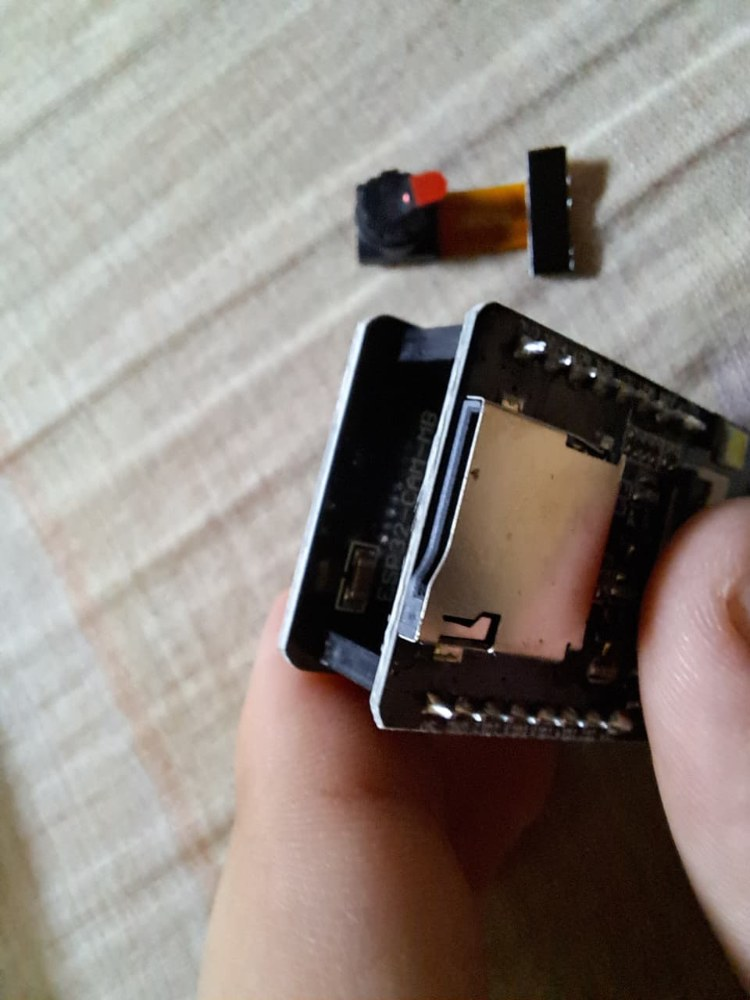
\includegraphics[height=5.4cm]{photos/esp32cam_assemblage.jpg}
  \caption{Assemblage des deux cartes}
\end{subfigure}
\caption{Module ESP32-CAM et son support ESP32-CAM-MB}
\label{fig:esp32cam}
\end{figure}

La caméra exécute le programme d'exemple \textit{CameraWebServer} d'Espressif. Celui-ci se connecte au réseau Wi-Fi
local et expose deux services HTTP : un flux vidéo MJPEG sur le port 81 (\texttt{/stream}) et une interface de
réglage sur le port 80 (\texttt{/status}, \texttt{/control}) pour la résolution, la qualité JPEG, le flash, le
retournement ou le miroir de l'image. Nous utilisons la résolution VGA (640\,$\times$\,480).

Deux particularités du montage ont eu des conséquences sur le logiciel :
\begin{itemize}
  \item \textbf{L'adresse IP est attribuée dynamiquement} par le point d'accès. Le serveur retrouve donc la caméra
        automatiquement (dernière adresse connue, puis balayage du sous-réseau), comme décrit au chapitre~4.
  \item \textbf{La caméra est montée sur la tranche}, à l'avant droit de la voiture : l'image arrive tournée de
        90°. Le capteur ne sait que retourner ou inverser l'image ; la rotation est donc réalisée par le serveur
        avant l'affichage et la détection.
\end{itemize}

% ------------------------------------------------------------------------------------------------
\section{Système d'alimentation}

L'alimentation du prototype est volontairement simple et repose sur deux sources séparées, sans circuit de
régulation supplémentaire (figure~\ref{fig:alimentation}) :
\begin{itemize}
  \item \textbf{quatre piles alcalines AA} de 1,5 V (Duracell), soit environ 6 V, reliées à l'entrée VS du L298N à
        travers un interrupteur marche/arrêt : elles alimentent uniquement les moteurs ;
  \item \textbf{une batterie externe USB 5 V}, qui alimente la caméra ESP32-CAM par sa carte MB ainsi que
        l'électronique de commande. Le rail logique 5 V et la masse sont communs à l'Arduino, au L298N, au HC-SR04
        et aux deux capteurs infrarouges.
\end{itemize}

\begin{figure}[H]
\centering
\begin{subfigure}[b]{0.3\linewidth}\centering
  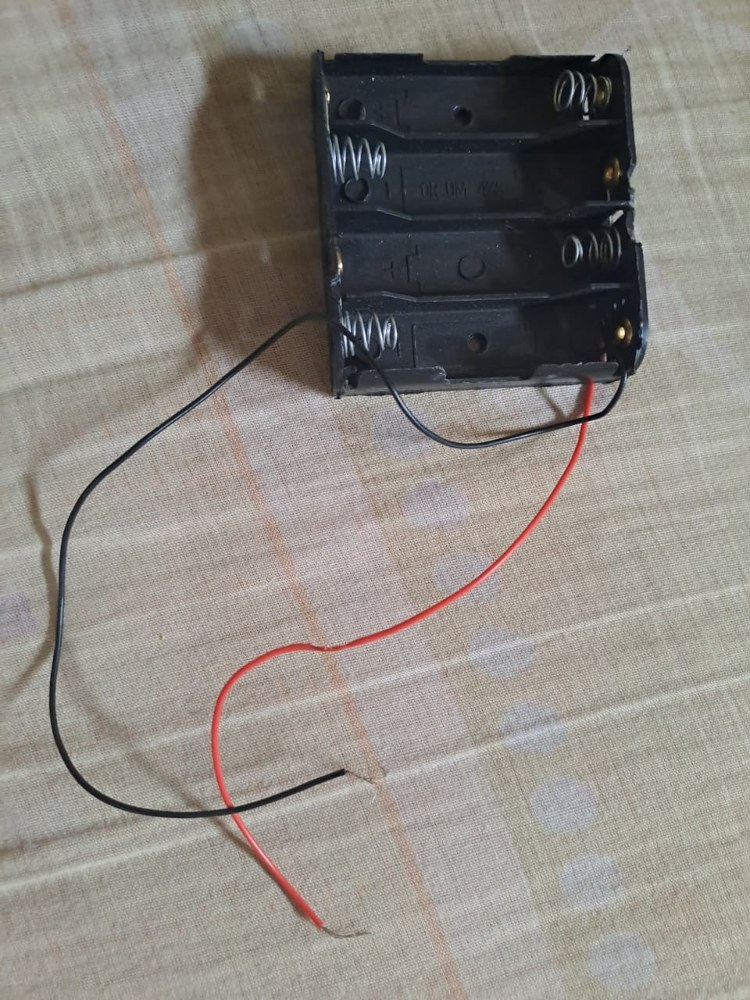
\includegraphics[height=4.6cm]{photos/piles_aa.jpg}
  \caption{Support de 4 piles AA}
\end{subfigure}\hspace{0.8cm}
\begin{subfigure}[b]{0.3\linewidth}\centering
  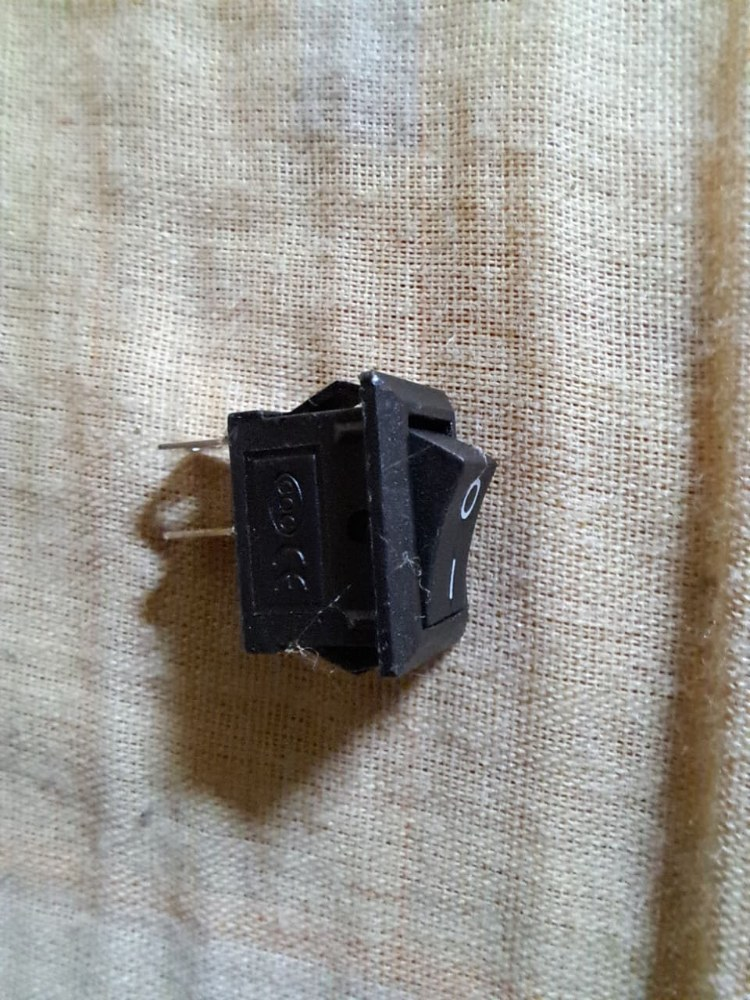
\includegraphics[height=4.6cm]{photos/interrupteur.jpg}
  \caption{Interrupteur marche / arrêt}
\end{subfigure}
\caption{Éléments du circuit d'alimentation des moteurs}
\label{fig:alimentation}
\end{figure}

Cette séparation est volontaire. Au démarrage et lors des changements de sens, les moteurs appellent des pointes
de courant qui font chuter la tension ; partagée avec la caméra, cette chute provoquerait des redémarrages de
l'ESP32 (\textit{brownout}), particulièrement sensible pendant les émissions Wi-Fi. Le tableau~\ref{tab:conso}
donne des ordres de grandeur des consommations.

\begin{table}[H]
\centering\small
\caption{Ordres de grandeur des consommations (valeurs typiques des fiches techniques)}
\label{tab:conso}
\begin{tabular}{lll}
\toprule
\textbf{Élément} & \textbf{Source} & \textbf{Consommation typique} \\
\midrule
2 moteurs TT & piles AA (via L298N) & 2 $\times$ 100 à 250 mA en roulage, davantage au démarrage \\
Arduino UNO & batterie USB & $\approx$ 50 mA \\
HC-SR04 & rail 5 V (Arduino) & $\approx$ 15 mA \\
2 capteurs IR & rail 5 V (Arduino) & 2 $\times$ $\approx$ 20 mA \\
ESP32-CAM (diffusion Wi-Fi) & batterie USB & $\approx$ 200 à 300 mA, plus avec le flash \\
\bottomrule
\end{tabular}
\end{table}

Cette solution a l'avantage de la simplicité : les piles se remplacent facilement et la batterie externe se
recharge par USB. Compte tenu de la chute de tension du L298N, une batterie lithium de 7,4 V permettrait
toutefois aux moteurs de recevoir une tension plus proche de leur valeur nominale et à la voiture d'aller plus
vite.

% ------------------------------------------------------------------------------------------------
\section{Schéma de câblage}

Le schéma de câblage complet est donné par la figure~\ref{fig:montage}, et le tableau~\ref{tab:liaisons} en
reprend les liaisons.

\begin{figure}[H]
\centering
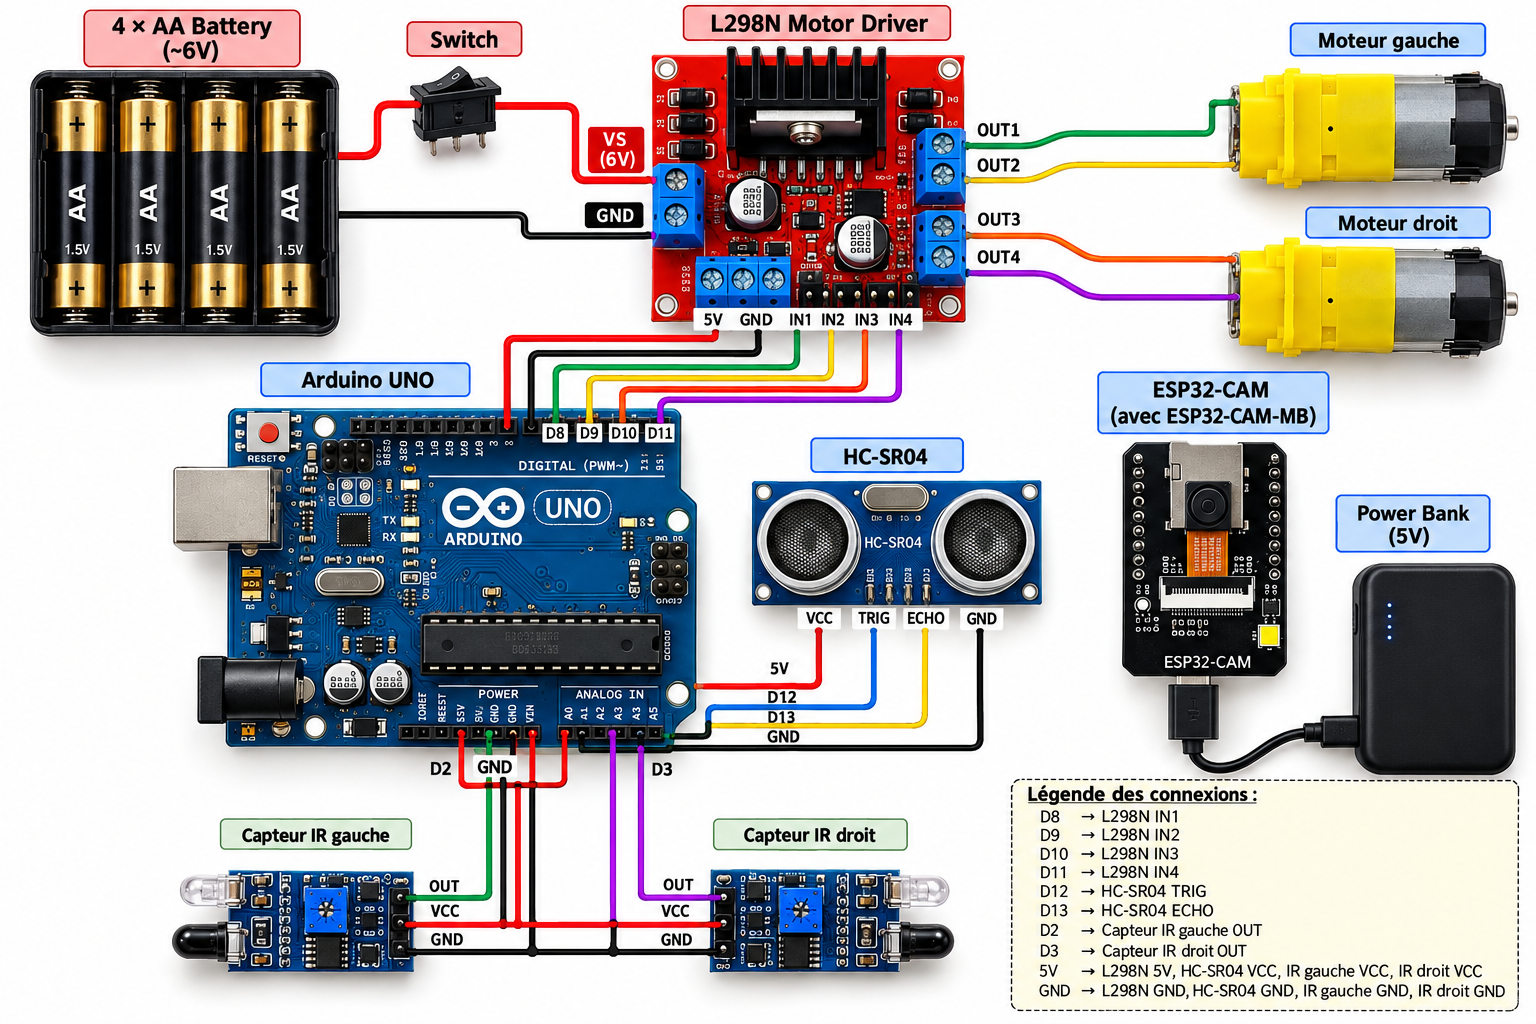
\includegraphics[width=\linewidth]{montage.png}
\caption{Schéma de câblage du prototype}
\label{fig:montage}
\end{figure}

\begin{table}[H]
\centering\small
\caption{Liaisons du schéma de câblage}
\label{tab:liaisons}
\begin{tabular}{ll}
\toprule
\textbf{De} & \textbf{Vers} \\
\midrule
Piles AA (+) $\rightarrow$ interrupteur & L298N VS (6 V) \\
Piles AA ($-$) & L298N GND \\
L298N OUT1, OUT2 / OUT3, OUT4 & Moteur gauche / moteur droit \\
Arduino D8, D9, D10, D11 & L298N IN1, IN2, IN3, IN4 \\
Arduino D12 / D13 & HC-SR04 Trig / Echo \\
Arduino D2 / D3 & Sortie OUT du capteur IR gauche / droit \\
Arduino 5 V & L298N 5 V, HC-SR04 VCC, VCC des capteurs IR \\
Arduino GND & L298N GND, HC-SR04 GND, GND des capteurs IR \\
Batterie externe (USB 5 V) & ESP32-CAM-MB $\rightarrow$ ESP32-CAM ; Arduino UNO (USB) \\
\bottomrule
\end{tabular}
\end{table}

% ------------------------------------------------------------------------------------------------
\section{Réalisation physique du prototype}

Le prototype est monté sur un châssis en acrylique à deux roues motrices et une roue folle
(figure~\ref{fig:chassis}). Les composants sont disposés pour garder un centre de gravité bas et laisser à la
caméra un champ de vision dégagé (figure~\ref{fig:prototype}) :
\begin{itemize}
  \item à l'avant, le HC-SR04 est fixé au centre du pare-chocs, encadré par les deux capteurs infrarouges orientés
        vers le sol, à quelques millimètres de la piste ;
  \item l'ESP32-CAM, montée sur la tranche avec sa carte MB, occupe l'angle avant ; sa caméra regarde vers
        l'avant, à hauteur de la piste, ce qui donne le point de vue d'un conducteur ;
  \item l'Arduino UNO est placé au centre du châssis, l'interrupteur juste derrière ;
  \item à l'arrière, la batterie externe porte le module L298N, au plus près des moteurs.
\end{itemize}

\begin{figure}[H]
\centering
\begin{subfigure}[b]{0.38\linewidth}\centering
  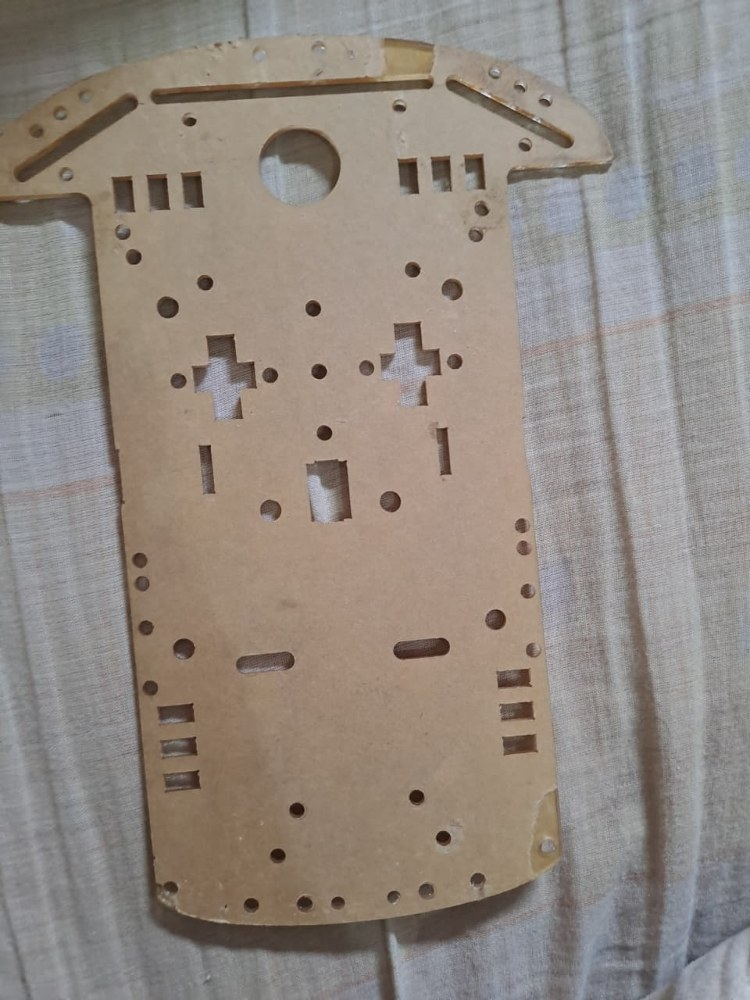
\includegraphics[height=5cm]{photos/chassis.jpg}
  \caption{Châssis en acrylique}
\end{subfigure}\hspace{0.8cm}
\begin{subfigure}[b]{0.38\linewidth}\centering
  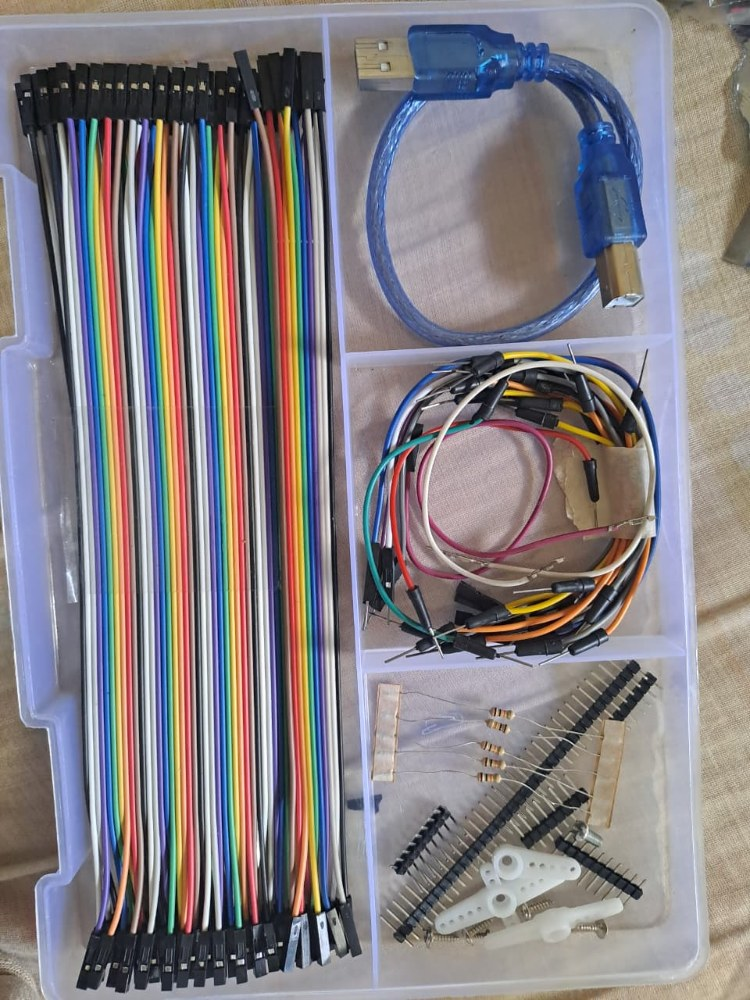
\includegraphics[height=5cm]{photos/fils_dupont.jpg}
  \caption{Fils de liaison Dupont}
\end{subfigure}
\caption{Éléments mécaniques et de liaison}
\label{fig:chassis}
\end{figure}

\begin{figure}[H]
\centering
\begin{subfigure}[b]{0.49\linewidth}\centering
  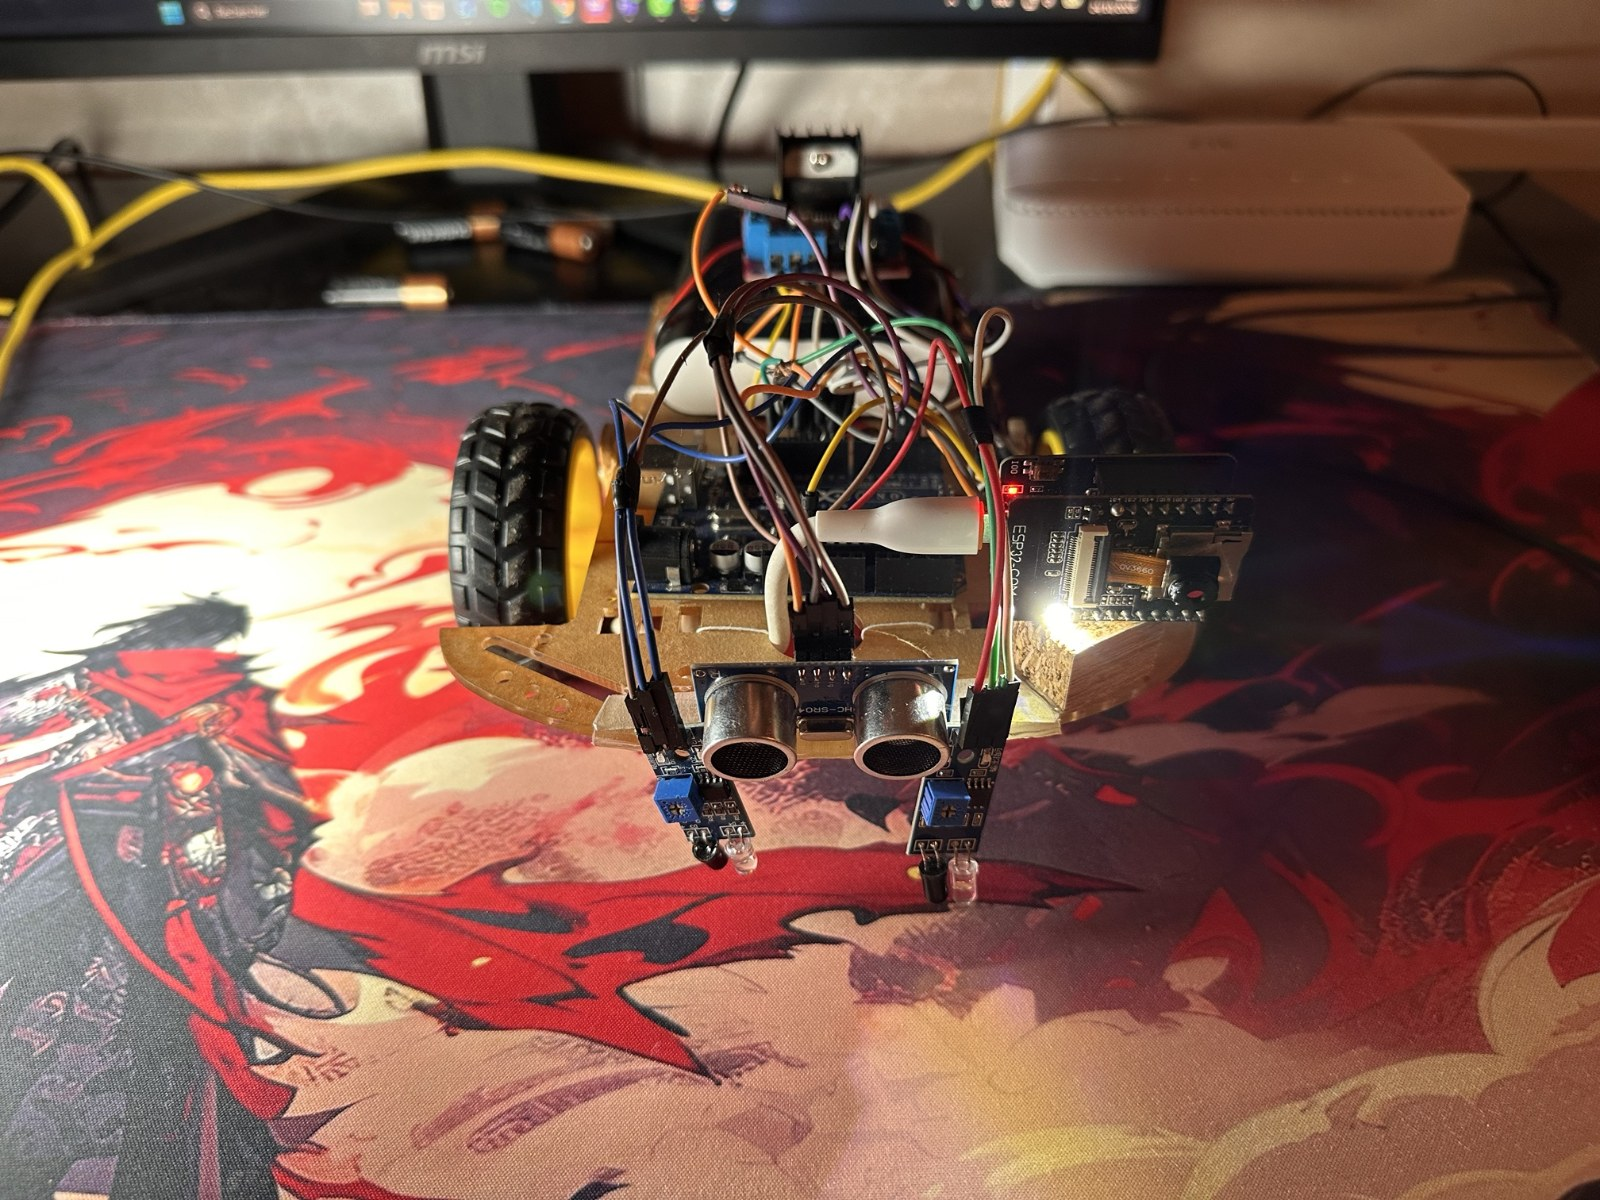
\includegraphics[width=\linewidth]{photos/prototype_avant.jpg}
  \caption{Vue avant : HC-SR04, capteurs IR et ESP32-CAM}
\end{subfigure}\hfill
\begin{subfigure}[b]{0.49\linewidth}\centering
  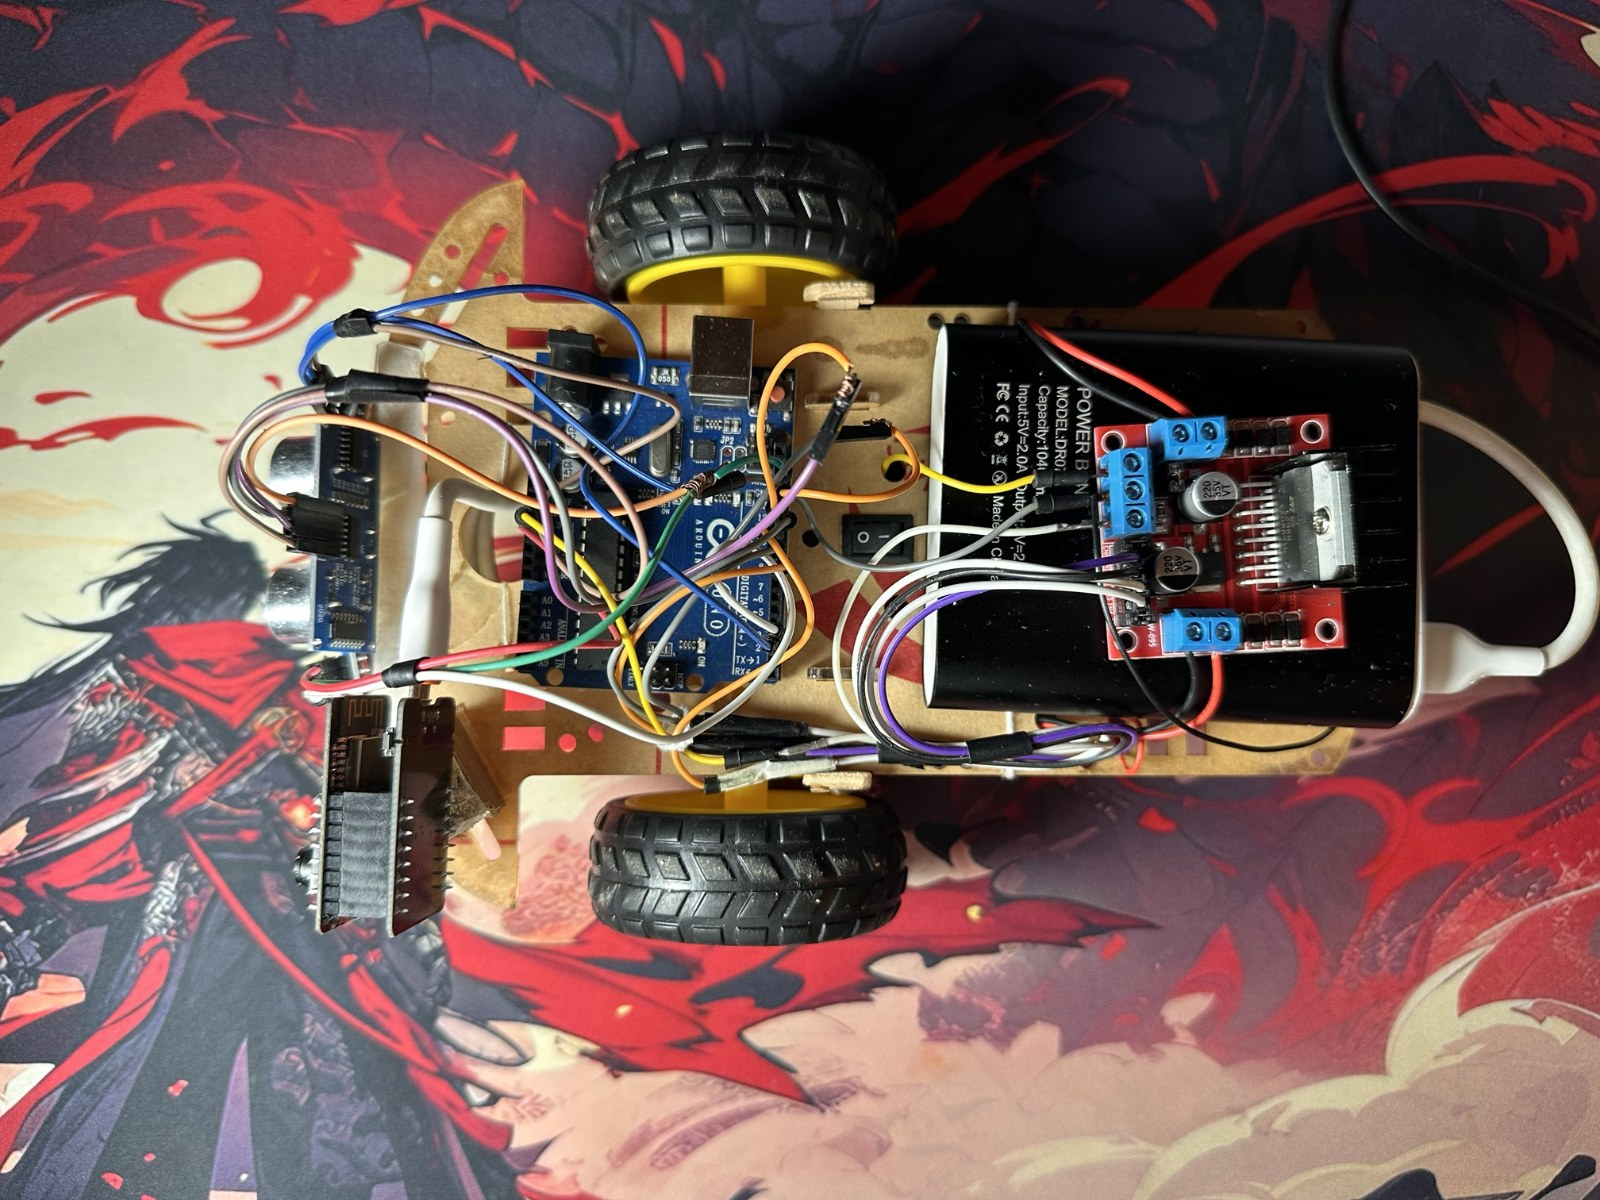
\includegraphics[width=\linewidth]{photos/prototype_dessus.jpg}
  \caption{Vue de dessus : Arduino, L298N et batterie externe}
\end{subfigure}
\caption{Prototype assemblé}
\label{fig:prototype}
\end{figure}

\subsection*{Logique de commande embarquée}
Le programme de l'Arduino combine le suivi de ligne et la sécurité frontale. À chaque itération, il mesure la
distance frontale ; si un obstacle est trop proche, il arrête les moteurs, sinon il applique la logique de suivi
de ligne du tableau~\ref{tab:suivi}. L'algorithme~\ref{alg:commande} en résume le principe.

\begin{algorithm}[H]
\caption{Principe de la boucle de commande de l'Arduino}
\label{alg:commande}
\begin{algorithmic}[1]
\Loop
  \State $d \gets$ distance mesurée par le HC-SR04
  \If{$d < d_{\text{sécurité}}$} \State arrêter les deux moteurs \Comment{obstacle devant la voiture}
  \Else
    \State $g \gets$ état du capteur IR gauche, \ $r \gets$ état du capteur IR droit
    \If{$g = $ sol clair \textbf{et} $r = $ sol clair} \State avancer
    \ElsIf{$g = $ ruban} \State tourner à gauche \Comment{moteur gauche ralenti}
    \ElsIf{$r = $ ruban} \State tourner à droite \Comment{moteur droit ralenti}
    \Else \State s'arrêter
    \EndIf
  \EndIf
\EndLoop
\end{algorithmic}
\end{algorithm}

\subsection*{Piste d'essai}
La piste est une boucle fermée tracée au ruban adhésif noir sur un carrelage clair, aux angles arrondis
(figure~\ref{fig:piste}). Ses dimensions ne sont pas figées : la piste est retracée à chaque séance d'essai selon
l'espace disponible, et sa géométrie peut être redéfinie dans l'éditeur de piste de l'application. Deux obstacles
y sont placés : une \textbf{colonne} rayée à sommet noir
et une \textbf{boîte} de couleur crème. Ce sont les deux classes que le modèle du prototype doit reconnaître
(chapitre~3). Les six points de passage A à F de la piste, définis dans l'application, peuvent recevoir des
marqueurs ArUco imprimés que la caméra lit pour localiser la voiture.

\begin{figure}[H]
\centering
\begin{subfigure}[b]{0.52\linewidth}\centering
  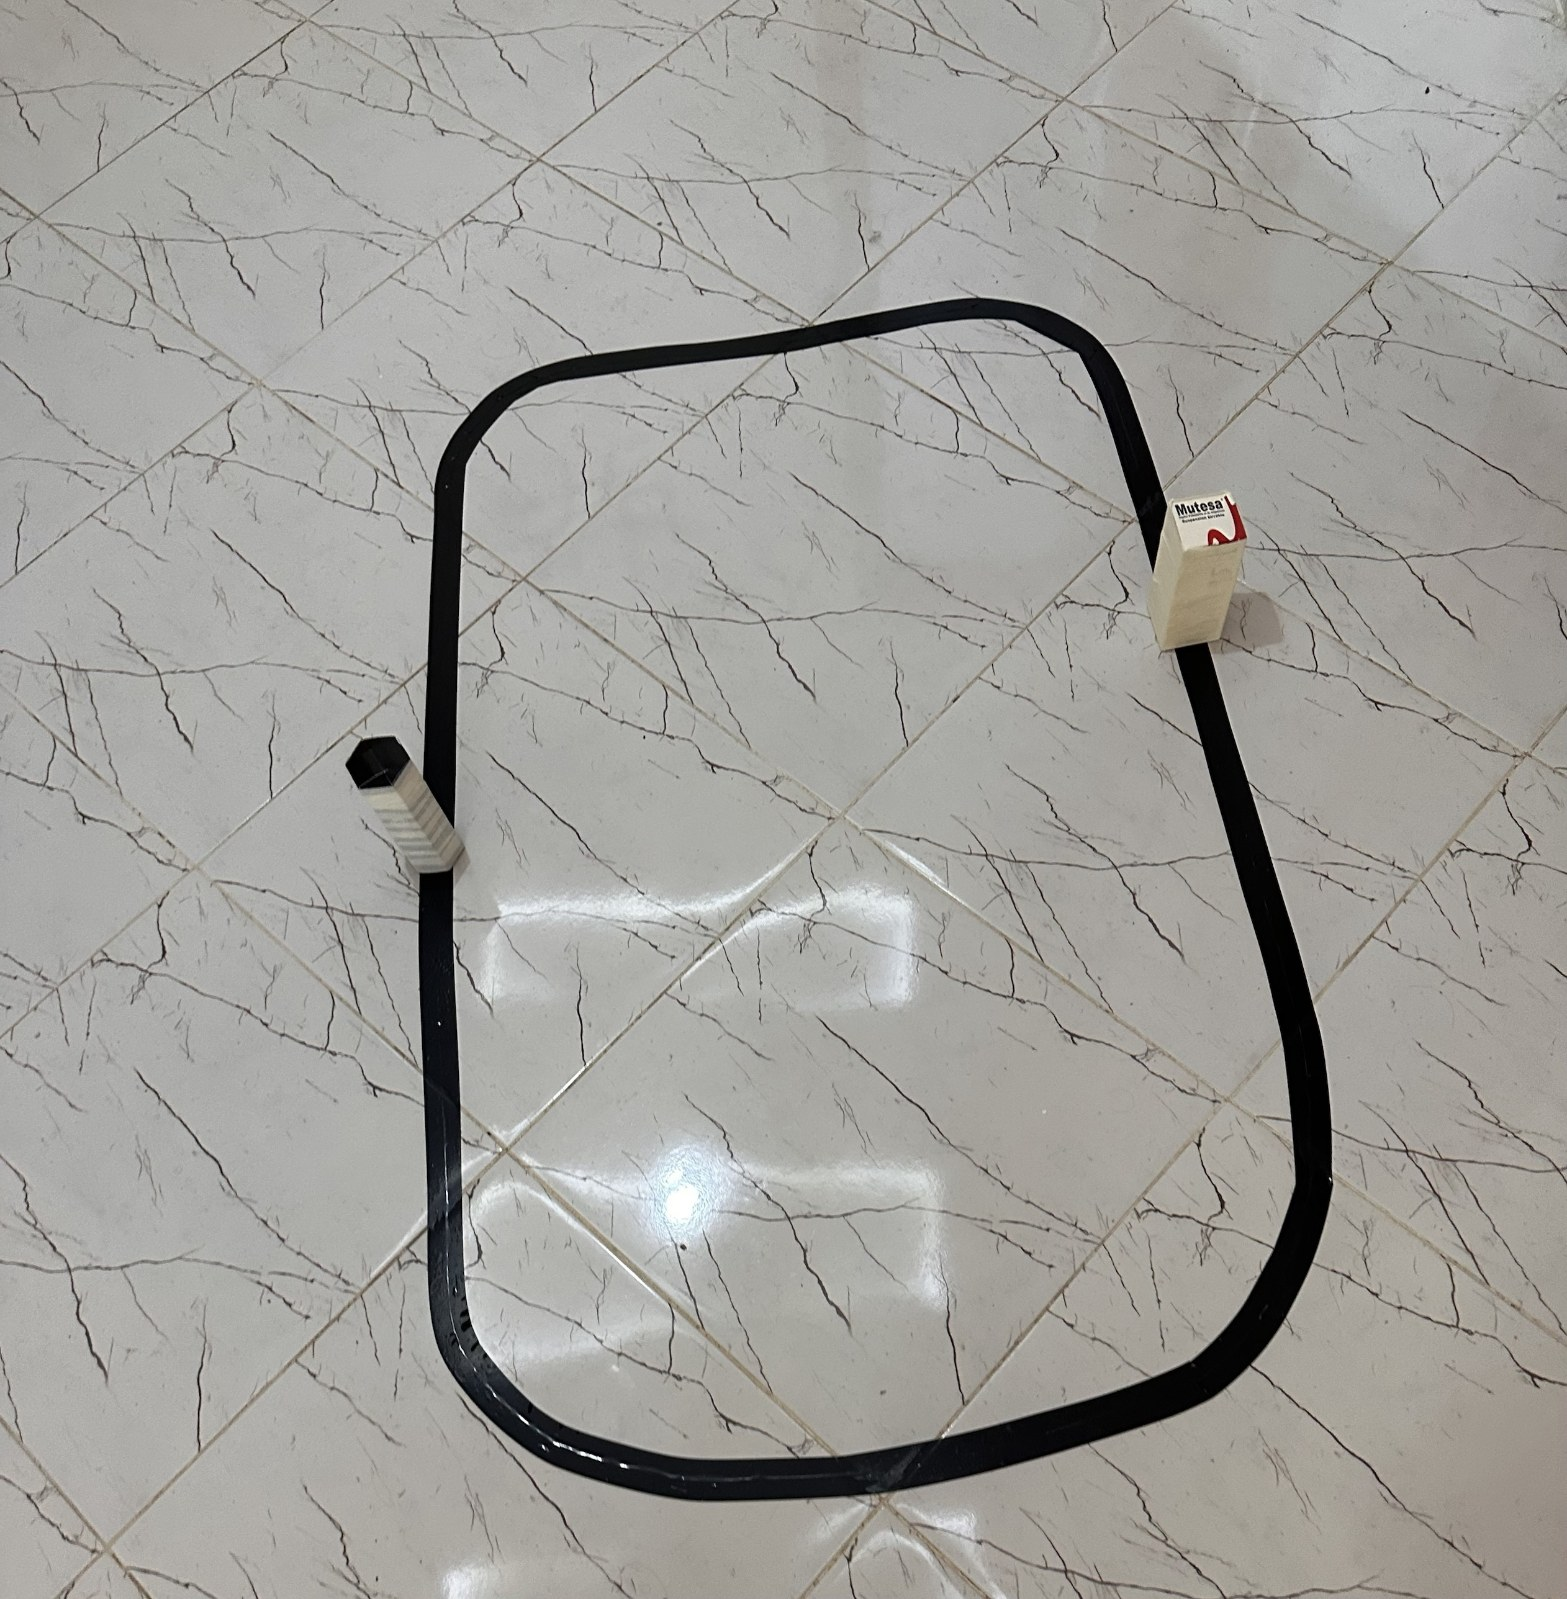
\includegraphics[height=7.2cm]{photos/piste.jpg}
  \caption{Vue de dessus de la piste et des deux obstacles}
\end{subfigure}\hfill
\begin{subfigure}[b]{0.42\linewidth}\centering
  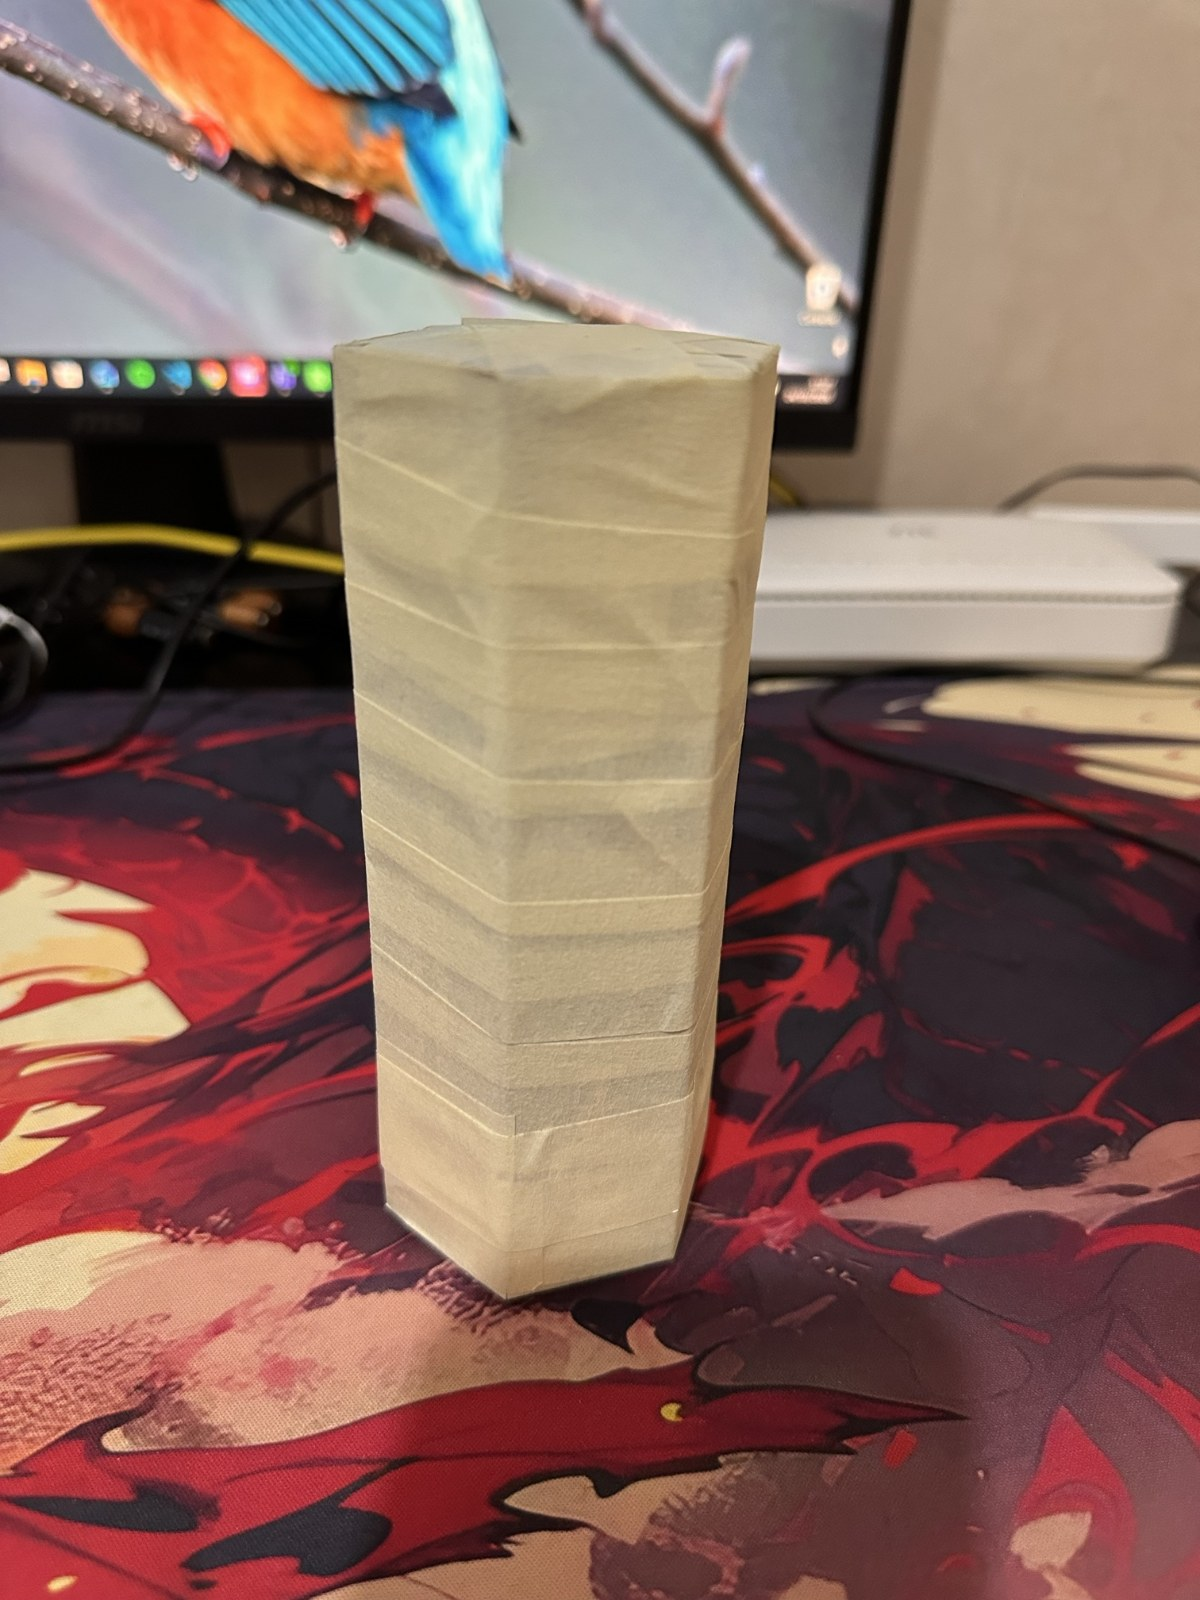
\includegraphics[height=7.2cm]{photos/obstacle_colonne.jpg}
  \caption{Obstacle « colonne »}
\end{subfigure}
\caption{Piste d'essai et obstacles du prototype}
\label{fig:piste}
\end{figure}

\chapconclusion
Ce chapitre a présenté la réalisation matérielle du prototype : une architecture en deux sous-systèmes
indépendants, l'un pour la commande (Arduino, L298N, moteurs, capteurs infrarouges et ultrasonique), l'autre pour la
vision (ESP32-CAM). Le prototype suit sa piste de façon autonome et fournit, par sa caméra, les images que les
modèles d'intelligence artificielle du chapitre suivant vont analyser.
